        \chapter{Methodology and Solution Proposal}
        \label{chap:Chapter3}

        The migration of critical software infrastructure from C++ to Rust is not a
        syntactic translation exercise but a fundamental architectural transformation.
        It requires rethinking ownership, concurrency, and interface boundaries in order
        to preserve functionality while improving safety guarantees.

        As discussed in Chapter \ref{chap:Chapter2}, the so-called ``Boost Paradox''
        introduces a unique challenge: the very features that make Boost powerful—such as
        templates and metaprogramming—also hinder the applicability of automated
        interoperability tools.

        This chapter defines a structured methodology to decompose Boost-based systems
        and proposes an architectural design that incrementally bridges the safety gap
        between C++ and Rust.

        \section{Component Selection Criteria}
        \label{sec:SelectionCriteria}

        Historically, a ``big bang'' rewrite of large C++ codebases into Rust has proven
        prone to failure due to the difficulty of verifying feature parity, the
        disruption of ongoing development, and the elevated certification risk in
        safety-critical domains. Consequently, this research adopts a selective and
        incremental migration strategy.

        Boost libraries are not considered uniformly; instead, they are evaluated and
        selected based on their relevance, isolation capability, and suitability for
        automotive software architectures.

        \subsection{Automotive-Oriented Selection Rationale}

        The automotive sector has increasingly adopted open-source and modular software
        platforms to address growing system complexity and multi-vendor integration. In
        this context, several automotive manufacturers and suppliers participate in
        Eclipse Software Defined Vehicle initiatives, including Eclipse \gls{SCORE}.

        Eclipse \gls{SCORE} is an open-source automotive platform initiative focused on a shared
        foundation for software-defined vehicles and high-performance ECUs, with safety and
        standards alignment forming part of its development context \parencite{eclipse_score}. These initiatives reflect the
        realities of modern automotive development: large, heterogeneous C++ codebases,
        long product lifecycles, and strict constraints on timing, memory usage, and
        failure modes. Such characteristics render wholesale language replacement
        infeasible and reinforce the need for incremental, well-contained migration
        strategies.

        The Boost libraries selected for migration are therefore evaluated according to
        the following automotive-oriented criteria:

        \begin{itemize}
        \item \textbf{Relevance to in-vehicle software}: Preference is given to
        libraries commonly used in middleware, communication, configuration
        management, and concurrency control, which are prevalent in automotive
        Electronic Control Units (ECUs) and service-oriented vehicle architectures.

        \item \textbf{Deterministic behavior}: Libraries whose runtime behavior is
        predictable and suitable for real-time or near-real-time constraints are
        prioritized, aligning with automotive requirements for bounded latency and
        reproducible execution.

        \item \textbf{Safety and robustness}: Components that encode disciplined
        resource management or concurrency patterns (e.g., Boost.SmartPtr,
        Boost.Thread, Boost.Asio) are preferred, as they conceptually align with
        Rust’s ownership and concurrency models.

        \item \textbf{Isolation capability}: Libraries that can be encapsulated
        behind stable, well-defined interfaces are favored, allowing them to serve
        as clear boundaries for Foreign Function Interface (FFI) integration.

        \item \textbf{Industrial and ecosystem relevance}: Libraries and migration patterns
        that are meaningful for open automotive software ecosystems, including Eclipse
        \gls{SCORE}, are preferred because they provide a concrete architectural context
        for evaluating incremental interoperability and portability.
        \end{itemize}

        \subsection{Operational Selection Criteria and Assessment}
        \label{sec:selection_assessment}

        The criteria above are converted into an explicit assessment procedure so that component selection is traceable rather than based only on qualitative intuition. Each candidate is assessed against the following dimensions: automotive relevance, safety relevance, isolation capability, interoperability constraints, portability relevance, performance relevance, implementation complexity, and suitability for exposing reusable migration patterns.

        Each dimension is rated on a five-point ordinal scale, where 1 indicates low relevance to the migration objective and 5 indicates high relevance. The scale is used as a structured decision aid rather than as an objective measurement of library quality. The assessment is documented before implementation so that the selection is not driven by the implementation results.

        \begin{table}[H]
        \centering
        \renewcommand{\arraystretch}{1.2}
        \begin{tabularx}{\textwidth}{|l|c|X|}
        \hline
        \textbf{Criterion} & \textbf{Weight} & \textbf{Assessment question} \\ \hline
        Automotive relevance & 15\% & Is the functionality relevant to low-level or embedded automotive software? \\ \hline
        Safety relevance & 15\% & Does the component expose memory, representation, ownership, or other safety-relevant concerns? \\ \hline
        Isolation capability & 15\% & Can the functionality be encapsulated behind a stable interface? \\ \hline
        Interoperability relevance & 15\% & Does the component expose meaningful Rust/C++ boundary-design challenges? \\ \hline
        Portability relevance & 10\% & Does the component involve platform, compiler, representation, or architecture concerns? \\ \hline
        Performance relevance & 10\% & Can meaningful performance characteristics be evaluated experimentally? \\ \hline
        Implementation complexity & 10\% & Is the component complex enough to exercise the methodology but bounded enough for a dissertation case study? \\ \hline
        Pattern generalisability & 10\% & Does the component expose migration decisions that can be separated from library-specific details? \\ \hline
        \end{tabularx}
        \caption{Operational criteria used for Boost component selection}
        \label{tab:selection_criteria}
        \end{table}

        Applying these criteria to the selected case studies gives the following qualitative assessment. The values are included to make the selection rationale explicit; they should not be interpreted as a universal ranking of Boost libraries.

        \begin{table}[H]
        \centering
        \renewcommand{\arraystretch}{1.2}
        \begin{tabular}{|l|c|c|}
        \hline
        \textbf{Criterion} & \textbf{Boost.Align} & \textbf{Boost.Endian} \\ \hline
        Automotive relevance & 4 & 4 \\ \hline
        Safety relevance & 5 & 5 \\ \hline
        Isolation capability & 5 & 5 \\ \hline
        Interoperability relevance & 5 & 5 \\ \hline
        Portability relevance & 4 & 5 \\ \hline
        Performance relevance & 5 & 4 \\ \hline
        Implementation complexity & 4 & 4 \\ \hline
        Pattern generalisability & 5 & 5 \\ \hline
        \end{tabular}
        \caption{Qualitative assessment of the selected Boost libraries}
        \label{tab:selected_library_assessment}
        \end{table}

        The two libraries were retained because they expose complementary migration problems rather than because they represent the largest or most template-heavy Boost components. Boost.Align concentrates on alignment, allocation, raw-pointer access, SIMD, and a C++03 compatibility boundary. Boost.Endian concentrates on binary representation, fixed-width values, generic abstractions, and a higher-level C++ interoperability mechanism. Together, these characteristics expose different points in the migration design space while remaining sufficiently bounded for controlled experimentation.

        \subsection{Boost.Align and Boost.Endian as Migration Enablers}
        \label{sec:migration_enablers}

        The purpose of selecting Boost.Align and Boost.Endian is not to claim that they are representative of every complex Boost library. Instead, they are treated as \textbf{migration-enabling case studies}: each exposes a set of lower-level problems that must be solved before the methodology can be applied confidently to larger or more template-heavy components.

        Boost.Align exposes patterns for representing alignment requirements, controlling ownership of allocated memory, isolating raw-pointer operations, defining opaque interfaces, and preserving interoperability with a C++03 consumer. Its implementation consequently provides a case study for translating memory-oriented C++ abstractions into Rust while keeping the unsafe surface explicit.

        Boost.Endian exposes a different set of patterns. Its conversion, buffer, and arithmetic layers require explicit reasoning about binary representation, fixed-width types, generic abstractions, and C++ interoperability. The implementation uses these characteristics to investigate how semantic behaviour can be retained without reproducing the original C++ template hierarchy literally.

        The resulting contribution is therefore the identification and evaluation of migration patterns rather than a claim that these two libraries solve the general Boost migration problem. The patterns that are potentially reusable include semantic rather than syntactic translation, explicit ownership contracts, isolation of unsafe operations, minimal FFI surfaces, and compatibility-driven selection of the interoperability mechanism. Decisions such as 32-byte alignment for the evaluated AVX workload or the use of a C ABI to preserve C++03 compatibility remain case-specific.

        \subsection{Deprioritized Components}

        Not all Boost libraries are suitable for migration or interoperability with
        Rust. Libraries that rely heavily on advanced template metaprogramming,
        domain-specific embedded languages, or extensive compile-time code generation
        are deprioritized due to their limited analyzability and poor suitability for
        FFI-based integration.

        Similarly, libraries without a clear connection to the low-level concerns
        exercised by the automotive case-study context are not prioritized within the
        scope of this work. Eclipse \gls{SCORE} is used as a motivating ecosystem rather
        than as evidence that the selected Boost libraries are already used by S-CORE.

        \subsection{Safety-Critical Constraints and ISO 26262 Alignment}

        ISO-26262 requires that software architectures for automotive safety systems
        support freedom from interference, predictable execution, and systematic fault
        avoidance. Programming languages and libraries used in such systems must
        minimize undefined behavior, provide explicit ownership semantics, and enable
        static verification wherever possible \parencite{iso26262}.

        C++’s permissive memory model and reliance on developer discipline pose
        challenges when targeting higher \gls{ASIL} levels. In practice, Boost libraries
        are frequently employed in automotive systems to impose structure and
        consistency on C++ development, particularly in resource management,
        concurrency, and asynchronous communication \parencite{synopsys_asil}.

        The proposed methodology leverages this disciplined use of Boost as a
        preparatory step toward Rust integration. By constraining C++ systems to
        well-defined Boost abstractions, reliance on raw pointers, implicit ownership
        conventions, and ad hoc concurrency mechanisms is reduced. This aligns with
        ISO-26262 recommendations for limiting systematic faults through controlled
        language subsets, coding guidelines, and architectural enforcement
        \parencite{iso26262}.

        Rust components introduced under this methodology are designed to maximize the use of Rust's static ownership and type guarantees. Where unsafe operations are necessary, they are isolated, documented, and treated as explicit safety-relevant boundaries. The methodology supports safety analysis and auditability, but the dissertation does not claim certification or a complete safety case.

        \subsection{Boost Libraries Relevant to Eclipse \gls{SCORE}}

        In Eclipse \gls{SCORE}-style automotive architectures, Boost libraries are
        commonly used to support middleware services, configuration management,
        concurrency, and asynchronous I/O. Their selection is driven by the need to
        enforce structure and predictability in large-scale, safety-relevant C++
        systems.

        Table~\ref{tab:boost_score_rust} summarizes Boost libraries commonly applicable
        to automotive platforms such as Eclipse \gls{SCORE} and their corresponding
        Rust-native equivalents.

        \begin{table}[h!]
        \centering
        \begin{tabular}{|l|l|p{6cm}|}
        \hline
        \textbf{Boost Library} & \textbf{Rust Equivalent} & \textbf{Automotive Relevance} \\ \hline

        Boost.Asio &
        \texttt{tokio}, \texttt{async-std} &
        Asynchronous I/O and event handling for in-vehicle services and middleware; requires careful runtime integration in safety-critical contexts \\ \hline

        Boost.Thread &
        \texttt{std::thread}, \texttt{crossbeam} &
        Thread management and synchronization for concurrent ECU software components \\ \hline

        Boost.SmartPtr &
        \texttt{Box}, \texttt{Rc}, \texttt{Arc} &
        Explicit ownership and lifetime management; directly maps to Rust’s ownership model \\ \hline

        Boost.Optional &
        \texttt{Option\textless T\textgreater} &
        Explicit representation of optional values, reducing NULL pointer usage \\ \hline

        Boost.Variant &
        \texttt{enum} &
        Type-safe sum types used in configuration, messaging, and state machines \\ \hline

        Boost.Program\_options &
        \texttt{clap}, \texttt{argh} &
        Configuration parsing for tooling and non-safety-critical control components \\ \hline

        Boost.Filesystem &
        \texttt{std::fs}, \texttt{std::path} &
        File and path handling in diagnostic, logging, and update subsystems \\ \hline

        Boost.Chrono &
        \texttt{std::time} &
        Time measurement and timeout handling with deterministic semantics \\ \hline

        \end{tabular}
        \caption{Boost libraries relevant to Eclipse SCORE–style automotive systems and Rust equivalents}
        \label{tab:boost_score_rust}
        \end{table}

        This mapping highlights that several Boost libraries already encode concepts
        such as explicit ownership, variant-based state, and structured concurrency—
        concepts that are native to Rust. As a result, the primary challenge of
        migration is architectural rather than conceptual, reinforcing the feasibility
        of incremental Rust adoption in safety-critical automotive ecosystems.

        \subsection{Comparative Analysis as a Migration Enabler}

        A central step in the proposed methodology is the comparison between Boost
        libraries used in automotive systems and their Rust-native equivalents. This
        comparison is not a simple replacement exercise, but an architectural analysis
        that exposes semantic gaps, safety assumptions, and ecosystem limitations.

        By explicitly mapping Boost abstractions to Rust constructs, developers can:
        \begin{itemize}
        \item Identify which safety properties are already enforced at the type level
        \item Detect mismatches in ownership, error handling, or concurrency semantics
        \item Quantify the residual risk that remains after migration
        \end{itemize}

        This analysis also reveals areas where no suitable Rust equivalent exists for
        automotive-grade use. In such cases, the absence of a mature Rust library becomes
        an explicit design signal rather than an implementation obstacle.

        \subsection{From Library Gaps to New Rust Automotive Crates}
        \label{subsec:NewRustLibraries}

        The comparison between Boost and Rust ecosystems frequently uncovers
        functionality that is either missing or insufficiently mature in Rust for
        safety-critical automotive contexts.

        Rather than forcing unsafe bindings or retaining C++ dependencies indefinitely,
        the proposed methodology treats these gaps as opportunities for new Rust library
        development. Such libraries are designed from the outset with:
        \begin{itemize}
        \item Explicit ownership and lifetime semantics
        \item Deterministic execution models suitable for real-time analysis
        \item Minimal and auditable unsafe code
        \item Alignment with AUTOSAR Adaptive concepts
        \end{itemize}

        In this sense, Boost serves not only as a migration bridge, but also as a
        functional benchmark that informs the evolution of Rust’s automotive ecosystem.
        The migration process thus becomes bidirectional: existing C++ designs guide
        Rust library development, while Rust’s guarantees inform safer architectural
        patterns in C++.

        \subsection{\gls{ASIL}-Oriented Migration Strategy}

        ISO-26262 distinguishes software components according to their
        \gls{ASIL}, ranging from \gls{QM} to \gls{ASIL}-D. Each level imposes increasing
        requirements on fault avoidance, fault detection, and freedom from interference.
        As a result, a uniform migration strategy is neither practical nor desirable
        across all \gls{ASIL} levels.

        The proposed methodology adopts a differentiated migration approach:

        \begin{itemize}
        \item \textbf{QM and \gls{ASIL}-A components}: Tooling, diagnostics, logging,
        configuration services, and non-safety-critical middleware. These components
        are suitable early candidates for Rust adoption, as certification
        constraints are less restrictive.

        \item \textbf{\gls{ASIL}-B and \gls{ASIL}-C components}: Communication services, resource
        managers, and coordination logic. Rust integration at this level focuses on
        reducing the exposure to memory-safety defects while evaluating execution-time behaviour.
        Unsafe Rust is strictly isolated and subject to additional verification.

        \item \textbf{\gls{ASIL}-D components}: Rust is introduced only where its guarantees
        provide demonstrable safety benefits. Components must be ownership-complete,
        free from dynamic allocation where required, and analyzable under
        \gls{WCET} constraints. \gls{FFI} boundaries are minimized and treated as
        safety-relevant interfaces subject to rigorous review.
        \end{itemize}

        This stratification aligns with ISO-26262 recommendations for mixed-criticality
        systems and supports freedom from interference between software elements of
        different ASIL levels.


        \subsection{Migration Workflow Overview}

        Figure \ref{fig:migration_workflow} presents the proposed incremental migration
        workflow for integrating Rust into Boost-based automotive software systems.
        The workflow is designed to support safety-critical development under
        ISO-26262 constraints while preserving system continuity and certification
        traceability.

        The process begins with a \textbf{comparative analysis} of existing Boost
        library usage and available Rust-native equivalents. This step establishes a
        semantic baseline by identifying ownership models, concurrency assumptions,
        error-handling mechanisms, and determinism properties already enforced in the
        C++ architecture.

        Based on this analysis, an \textbf{architectural refactoring phase} follows,
        during which Boost abstractions are used to constrain C++ components into
        well-defined, analyzable interfaces. This step reduces semantic ambiguity,
        limits undefined behavior, and prepares the system for language boundary
        introduction without altering functional behavior.

        Next, \textbf{\gls{FFI} boundary definition} is performed. Stable and minimal
        interfaces are identified between C++ and Rust components, with explicit
        ownership transfer rules and data lifetime guarantees. These boundaries are
        treated as safety-relevant interfaces and are subject to additional review
        and verification.

        The workflow then proceeds with \textbf{incremental Rust integration}, where
        Rust components are introduced selectively according to their assigned
        \gls{ASIL} level. Initial integration targets QM and ASIL-A components, followed
        by progressively higher-criticality elements as confidence, tooling maturity,
        and safety argumentation evolve.

        Throughout the process, \textbf{continuous verification and validation} are
        performed to ensure functional equivalence, timing predictability, and freedom
        from interference. Feedback from each iteration informs subsequent migration
        steps, allowing the workflow to adapt to architectural constraints and
        certification requirements.

        \begin{figure}[h!]
        \centering
        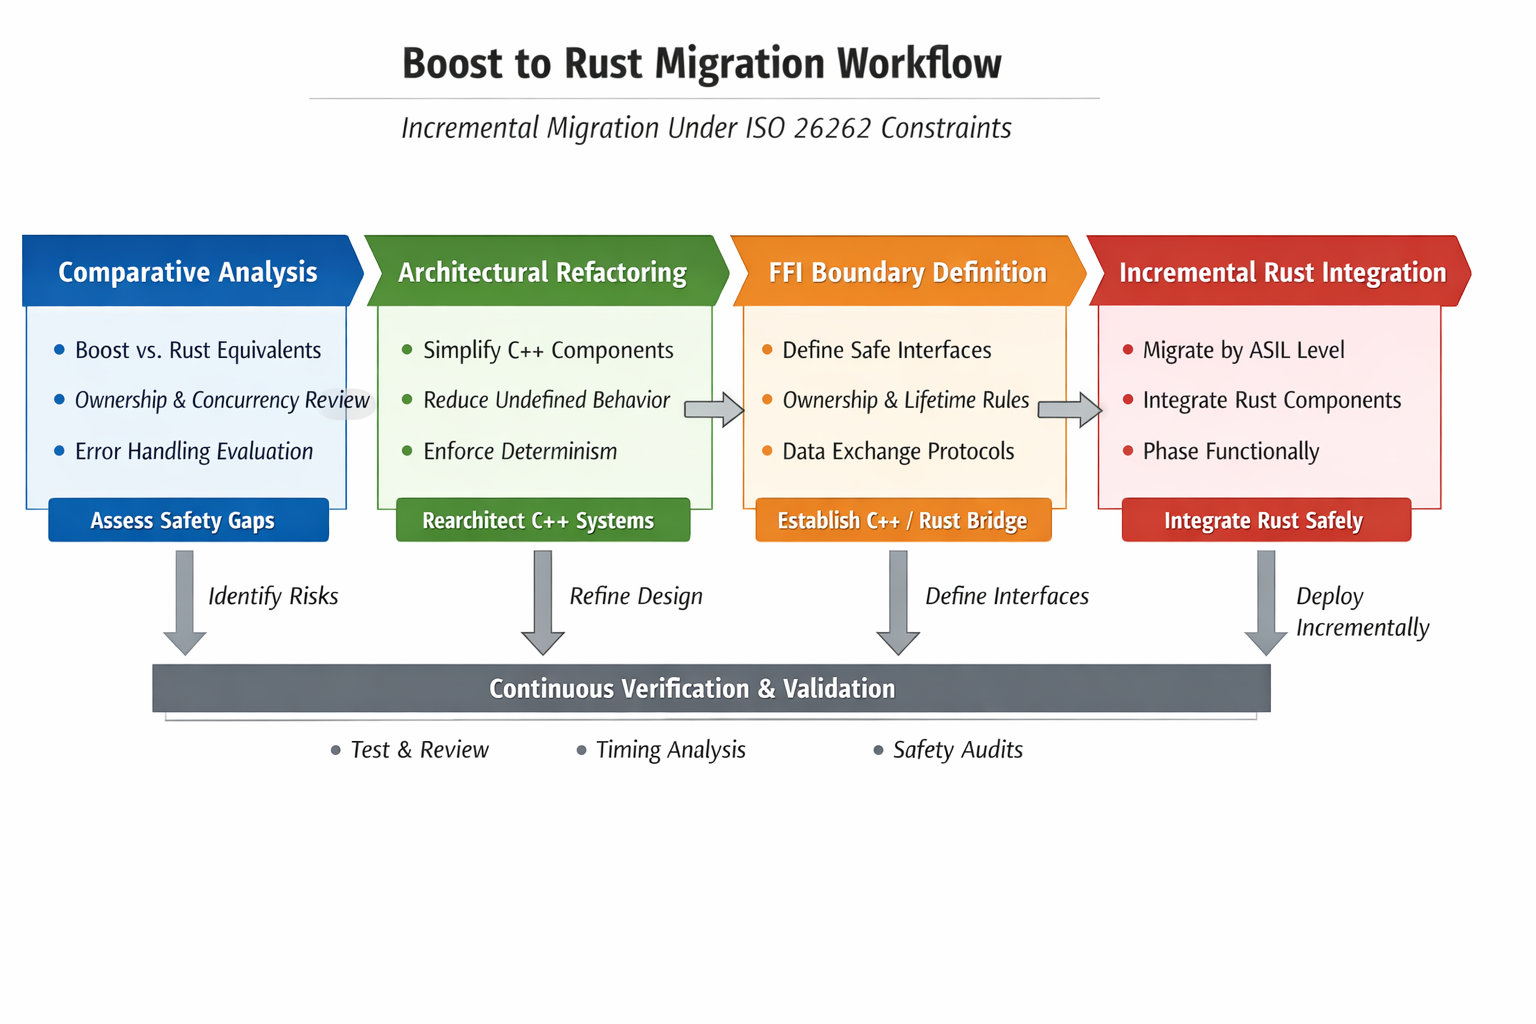
\includegraphics[width=0.9\textwidth]{ch3/assets/migration_workflow.png}
        \decoRule
        \caption[Boost-to-Rust Migration Workflow]{Incremental migration workflow for
        Boost-based automotive systems integrating Rust under ISO-26262 constraints}
        \label{fig:migration_workflow}
        \end{figure}

        Overall, the workflow emphasizes early reduction of semantic ambiguity on the
        C++ side and controlled introduction of Rust components, providing a more explicit
        interoperability boundary. Any claim of automotive safety compliance remains
        dependent on the complete system, development process, and applicable safety case.

\section{Research Design and Evaluation Plan}
\label{sec:research_design}

The proposed methodology is evaluated through two bounded case studies, \texttt{Boost.Align}
and \texttt{Boost.Endian}. The case-study design is intended to provide evidence about the
migration patterns identified by the methodology without implying that the results are
general measurements for all Boost libraries or all automotive software.

\subsection{Research Design}

Each case study follows the same high-level sequence: analysis of the original Boost
functionality, definition of equivalent Rust abstractions, implementation of the selected
functionality, integration through an appropriate FFI mechanism, functional validation,
and performance evaluation. This common structure makes it possible to distinguish
migration decisions that arise from the general methodology from those that are specific
to a library.

Boost.Align is used to evaluate low-level memory alignment, allocation, pointer handling,
SIMD-related operations, and compatibility with a C++03 consumer. Boost.Endian is used to
evaluate binary representation, fixed-width values, generic abstractions, and C++/Rust
interoperability through a higher-level interface. The two cases therefore exercise
complementary migration concerns while remaining sufficiently bounded for controlled
experimentation.

The automotive relevance is motivated by the requirements of modern software-defined
vehicle platforms. Eclipse S-CORE is an open-source automotive software platform aimed at
providing a shared foundation for high-performance ECUs and safety-critical vehicle
software, with emphasis on interoperability, portability, and automotive standards
\parencite{eclipse_score}. In this context, the selected libraries are not presented as
components that must be migrated in S-CORE itself. Instead, S-CORE is used as a motivating
architectural context in which incremental migration of low-level C++ infrastructure can
be relevant. The case studies consequently act as migration enablers: they expose
alignment, representation, ownership, and FFI patterns that can later inform work on
larger and more template-intensive components.

\subsection{Development Workflow}

The implementation follows four methodological phases: analysis; design and
implementation; interoperability; and validation and evaluation. The first phase
establishes the semantic baseline of the Boost implementation and identifies relevant
interfaces, ownership assumptions, dependencies, and observable behaviour. The second
phase defines Rust-native abstractions and implements the selected functionality without
requiring a literal translation of the C++ structure. The interoperability phase exposes
only the interface required by the existing C++ consumer. The final phase validates
functional behaviour and evaluates the measured characteristics of the resulting
implementation.

This workflow deliberately separates the conceptual methodology from the implementation
of each case study. The detailed migration procedure used within these phases is described
in Chapter~\ref{chap:Chapter4}, while the implementation and experimental results are
presented in Chapter~\ref{chap:Chapter6}.

\subsection{Validation and Evaluation Strategy}

Validation combines functional tests, interoperability checks, and benchmark measurements.
Functional validation verifies that the selected Rust functionality produces the expected
results for the evaluated inputs. Interoperability validation verifies that the exposed
interfaces can be consumed from the corresponding C++ environment. Performance evaluation
measures execution time and throughput for the workloads defined for each case study.

The evaluation is intentionally interpreted as experimental evidence for the selected
workloads. It does not establish worst-case execution time (WCET), jitter bounds,
schedulability, hard real-time guarantees, or a complete ISO 26262 safety case. Likewise,
process-level memory measurements are treated as observations of the benchmark process,
not as proof of lower memory consumption in general.

\subsection{Experimental Configuration}

The experiments use Rust 1.93 and Boost 1.91.0 as the implementation and reference
environments, respectively. Boost.Align is evaluated against a C++03-compatible interface,
while Boost.Endian uses the C++ interoperability mechanism selected for its implementation.
The benchmark configurations use release builds and repeated measurements; the reported
results are presented with the exact workload parameters in Chapter~\ref{chap:Chapter6}.

The evaluation focuses on three evidence categories: functional equivalence, measured
performance, and interoperability/safety-boundary characteristics. These categories are
sufficient to assess the feasibility of the proposed migration patterns while avoiding
claims that would require broader system-level experiments.

\subsection{Evaluation Scope and Limitations}

The selected case studies represent only a subset of Boost functionality. The results are
therefore used to evaluate the migration approach and identify practical trade-offs rather
than to generalize performance or safety properties to the complete Boost ecosystem.
In particular, the evaluation does not include complete vehicle-level integration,
long-duration operational testing, WCET analysis, multicore scheduling analysis, formal
verification, or certification assessment. These limitations are considered explicitly
when interpreting the results and the research questions in Chapter~\ref{chap:Chapter7}.

